\section{Múltiplas Categorias e TVD (Alameda County)}

\begin{frame}{Desafio de Múltiplas Categorias: Os Dados}
    \begin{block}{O Caso Alameda County (ACLU, 2010)}
        A ACLU avaliou o júri de 11 processos criminais ($1453$ pessoas no painel). É preciso determinar se a composição racial difere da população de forma sistemática.
    \end{block}
    
    \begin{columns}
        \begin{column}{0.48\textwidth}
            \begin{table}
                \centering
                \footnotesize
                \begin{tabular}{lcc}
                    \toprule
                    \textbf{Etnia} & \textbf{Elegível} & \textbf{Painel} \\
                    \midrule
                    Asiático & $0.15$ & $0.26$ \\
                    Negro & $0.18$ & $0.08$ \\
                    Branco & $0.54$ & $0.54$ \\
                    Hispânico & $0.12$ & $0.08$ \\
                    Outro & $0.01$ & $0.04$ \\
                    \bottomrule
                \end{tabular}
                \caption{Distribuição étnica}
            \end{table}
        \end{column}
        \begin{column}{0.52\textwidth}
            \centering
            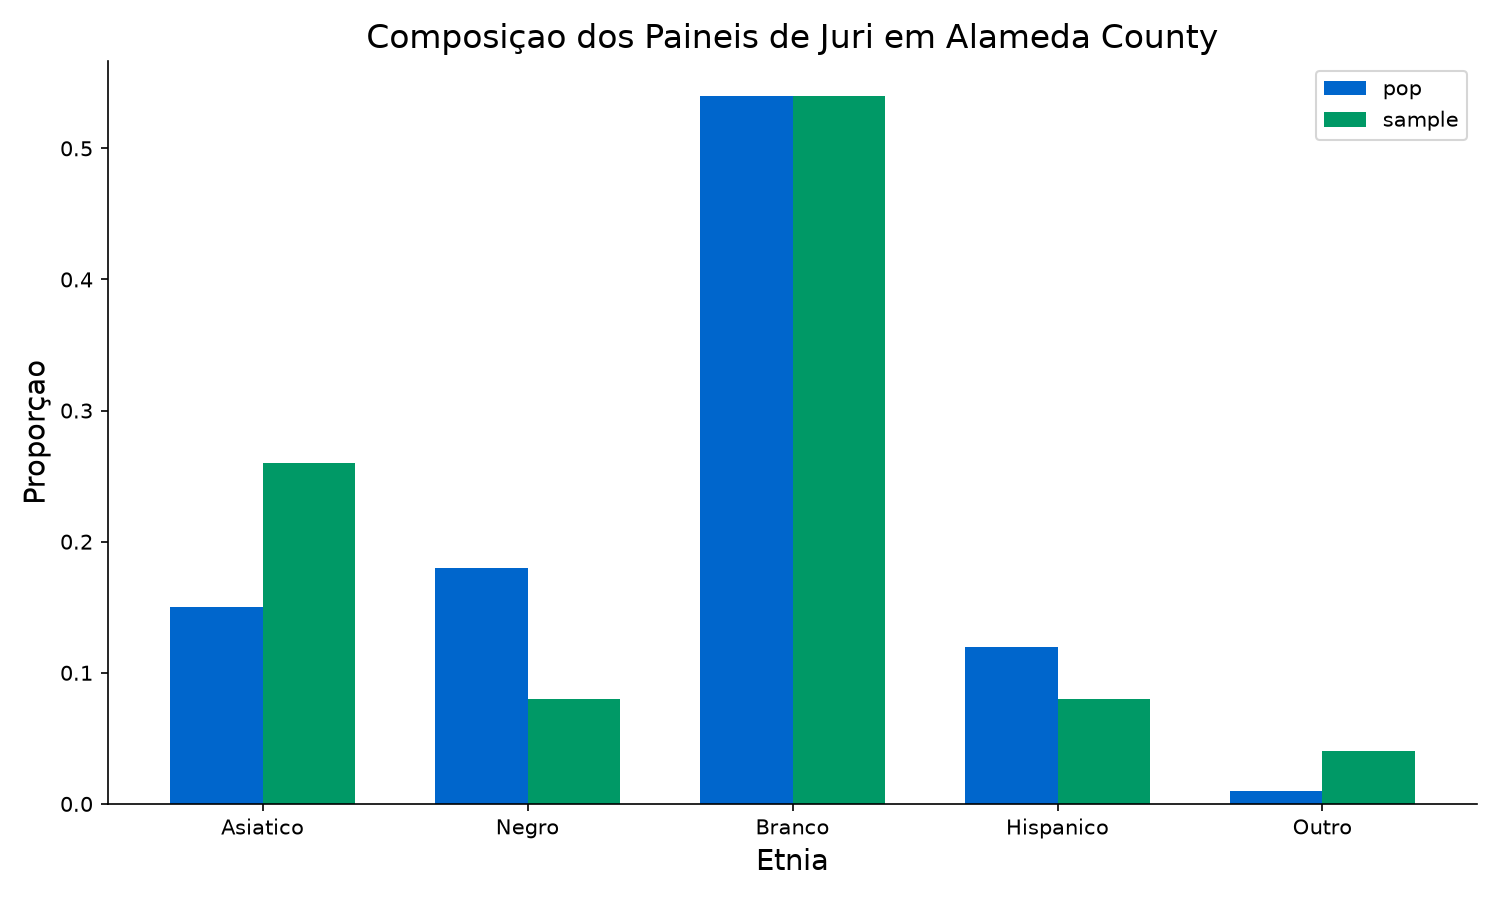
\includegraphics[width=\textwidth]{06_alameda_comparacao.png}
        \end{column}
    \end{columns}
\end{frame}

\begin{frame}{E se a Amostra Fosse Realmente Aleatória?}
    \begin{block}{Simulação de Seleção Justa (Amostra Multinomial)}
        Se o sorteio do júri de $1453$ pessoas fosse verdadeiramente aleatório e representativo, as proporções da amostra seriam muito próximas das proporções da população.
    \end{block}
    
    \begin{columns}
        \begin{column}{0.48\textwidth}
            \begin{table}
                \centering
                \footnotesize
                \begin{tabular}{lcc}
                    \toprule
                    \textbf{Etnia} & \textbf{Elegível} & \textbf{Aleatória} \\
                    \midrule
                    Asiático & $0.15$ & $0.14$ \\
                    Negro & $0.18$ & $0.18$ \\
                    Branco & $0.54$ & $0.56$ \\
                    Hispânico & $0.12$ & $0.11$ \\
                    Outro & $0.01$ & $0.01$ \\
                    \bottomrule
                \end{tabular}
                \caption{Amostra aleatória simulada}
            \end{table}
            \centering
            \vspace{0.1cm}
            {\footnotesize $TVD$ simulado: $0.0178$ ($1.78\%$)}
        \end{column}
        \begin{column}{0.52\textwidth}
            \centering
            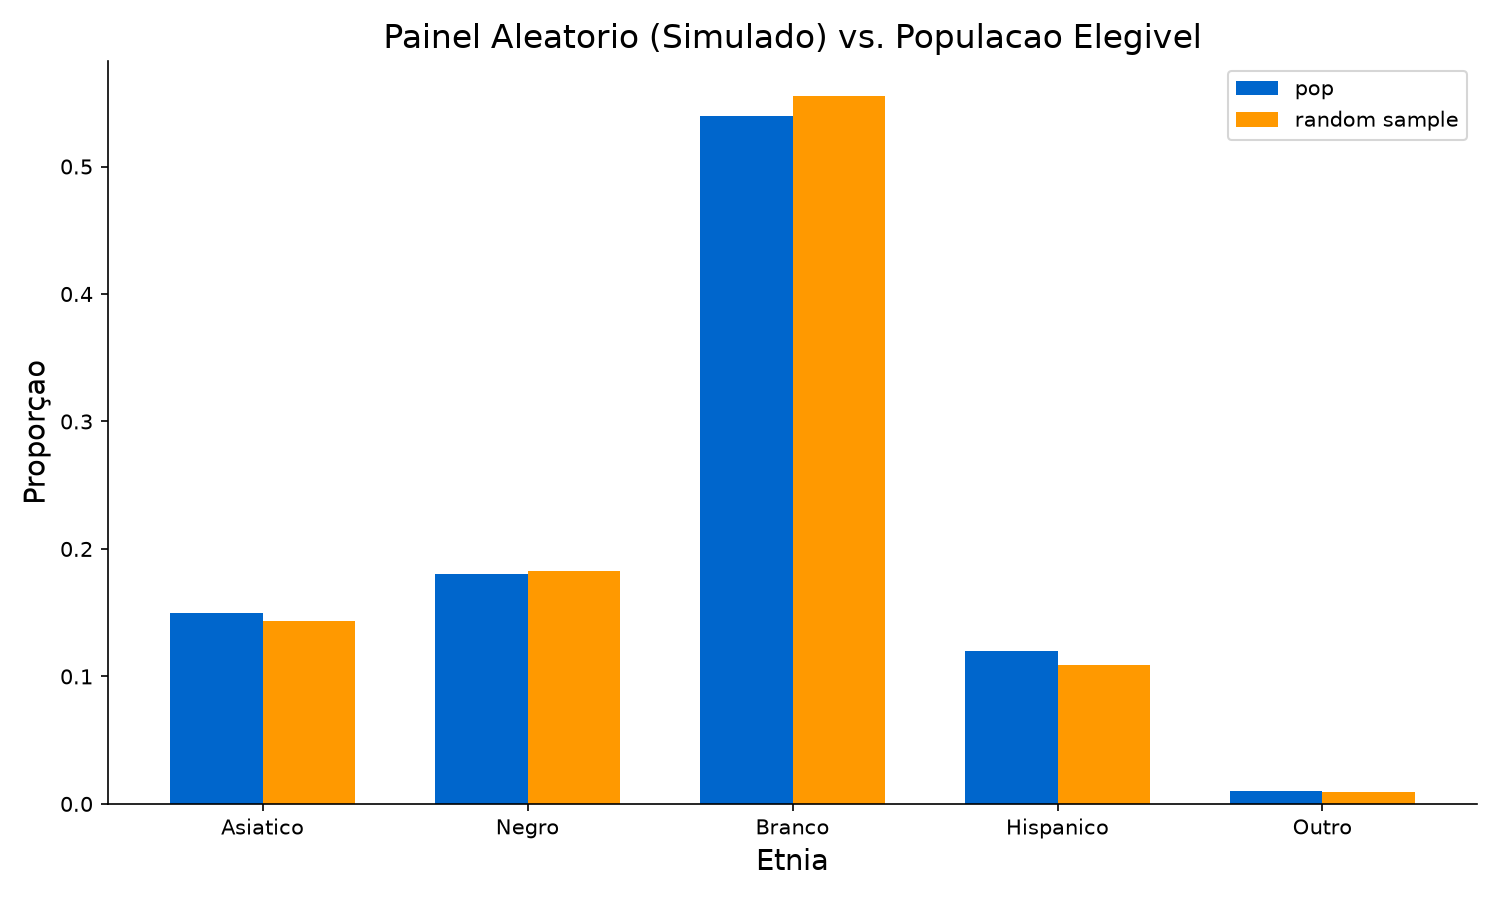
\includegraphics[width=\textwidth]{07_alameda_random_comparacao.png}
        \end{column}
    \end{columns}
\end{frame}

\begin{frame}{Matemática da Distância de Variação Total ($TVD$)}
    \begin{block}{Métrica de Distância de Variação Total ($TVD$)}
        Usada para comparar duas distribuições categóricas. É definida como metade da soma das diferenças absolutas entre as proporções de cada categoria:
        $$TVD = \frac{1}{2} \sum_{i=1}^{k} |p_i - q_i|$$
        Onde $p_i$ é a proporção amostral e $q_i$ é a proporção esperada.
    \end{block}
    \begin{block}{Exemplo de Cálculo para Alameda County:}
        {\small
        \begin{align*}
        TVD_{\text{obs}} = \frac{1}{2} \Big( &|0.26-0.15| + |0.08-0.18| + |0.54-0.54| + {} \\
        &|0.08-0.12| + |0.04-0.01| \Big) \\[1ex]
        TVD_{\text{obs}} = \frac{1}{2} \big( &0.11 + 0.10 + 0.00 + 0.04 + 0.03 \big) = \frac{0.28}{2} = 0.14
        \end{align*}
        }
    \end{block}
\end{frame}

\begin{frame}[fragile]{Abordagem Computacional: TVD}
\begin{lstlisting}[language=Python]
import numpy as np

prop_elegivel = np.array([0.15, 0.18, 0.54, 0.12, 0.01])
prop_painel = np.array([0.26, 0.08, 0.54, 0.08, 0.04])
obs_tvd = 0.5 * np.sum(np.abs(prop_painel - prop_elegivel))

tvds = []
np.random.seed(42)
for _ in range(10000):
    # Sorteia 1453 jurados de acordo com a distribuicao populacional
    amostra = np.random.multinomial(1453, prop_elegivel)
    prop_sim = amostra / 1453
    tvd_sim = 0.5 * np.sum(np.abs(prop_sim - prop_elegivel))
    tvds.append(tvd_sim)

# Calcula o P-valor
p_valor = np.count_nonzero(tvds >= obs_tvd) / 10000
print(f"P-valor: {p_valor}")
# Saida esperada: 0.0
\end{lstlisting}
\end{frame}

\begin{frame}{Alameda County: Decisão Visual}
    \begin{columns}
        \begin{column}{0.5\textwidth}
            \textbf{Análise do Gráfico:}
            \begin{itemize}
                \item Sob a hipótese nula, o $TVD$ máximo gerado em $10.000$ repetições foi próximo de $0.05$.
                \item O valor observado de $0.14$ está fora da região de variação aceitável do acaso.
                \item \textbf{Decisão:} Rejeitamos a hipótese nula $H_0$. O painel de Alameda County não foi selecionado aleatoriamente.
            \end{itemize}
        \end{column}
        \begin{column}{0.5\textwidth}
            \centering
            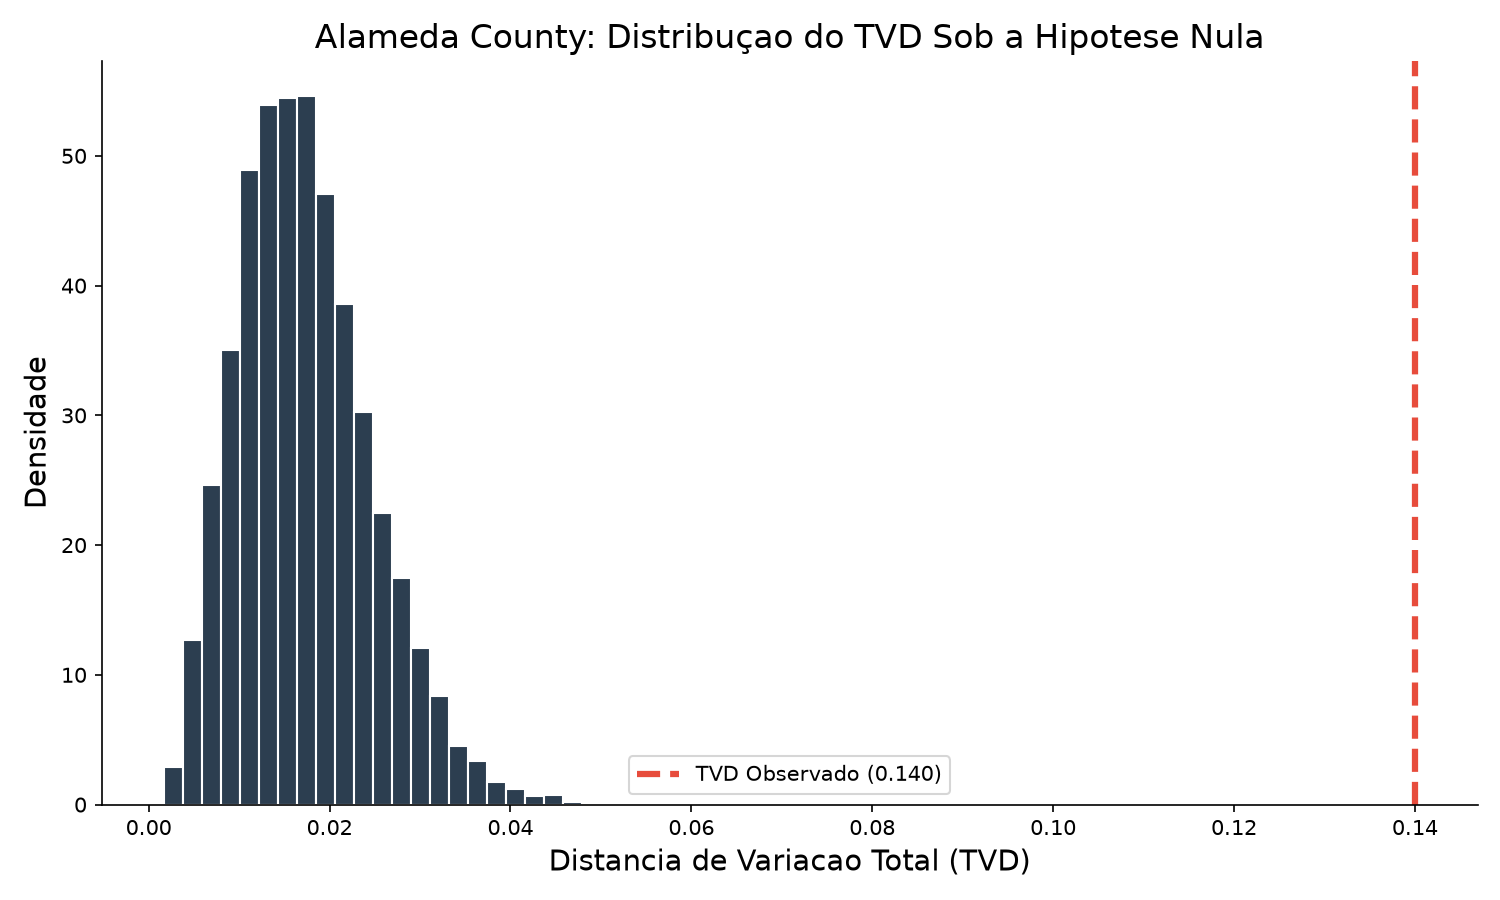
\includegraphics[width=\textwidth]{02_alameda_tvd.png}
        \end{column}
    \end{columns}
\end{frame}
